\section{Experiments}
\label{sec:experiments}
We answer the following questions in our experiments:
1. Sampling, Scaling, and Speeding.
2. Approximation Guarantees.
3. Budget vs. Infected.
4. Characterizing structure of the solution.

\subsection{Dataset and Methods}
We experiment with four very different kinds of networks, three random and one real, in order to fully explore the effect of network structure on the the results. We consider two random networks, namely the small world 
\cite{Kleinberg00thesmall-world}, and preferential attachment \cite{Barabasi509} models. Finally, we consider a synthetic agent based population for Montgomery County, VA, constructed by a first principles approach by \cite{barrett:wsc09,eubank:nature04}. This has been used in several public health studies, e.g., \cite{singh:bmc19}. This network has a rich set of demographic attributes for each node, e.g., age, gender, and income.

\noindent
\textbf{Methods.}
We use \algo{} with one time step (i.e., $\mathcal{T}=\{0\}$, also referred to as single stage), or two time steps (i.e., $\mathcal{T}=\{0, T\}$, referred to as two stage, with $t=0$ being the first stage, and $t=T$ being the second stage). For the single stage problem, we use the strategy of picking nodes based on highest degree or eigenscore, which is the component in the first eigenvector of the graph's adjacency matrix as baselines \cite{tong:cikm12}.
There are no prior baselines for temporal vaccination. 

\begin{table}[!h]
\centering
\begin{tabular}{llll}
\hline
 \textbf{Dataset} & \textbf{Nodes} & \textbf{Edges}   \\ \hline
 Montgomery & 70729 & 198138 \\
Preferential2 (PA2) & 100000 & 199996 \\
 Small World (SW) & 2500 & 14833 \\   
 Preferential1 (PA1) & 1000 & 1996 \\ \hline
\end{tabular}
\caption{Description of datasets}
\label{tab:datasets}
\end{table}

\subsection{Sampling, Scaling, and Speeding}
\textbf{Impact of varying $p$ on the average infections}
In this experiment, for each graph, we sample 100 subgraphs varying the probability of infection $p$. The expected number of sources are set to 10. Figure \ref{fig:PA_ar} shows, for the graph PA, that the average percentage of infections is low (within 30\% of the population) for $p \leq 0.25$, medium (within 60\%) for $0.25 < p < 0.4$, high ($\geq 60\%$) for $p \geq 0.4$. Figure \ref{fig:montgo_ar} shows that with a very small probability close to $0.1$, the average percentage of infections rise above 55\% (medium) of the total population. 

\begin{figure}[!h]
    \centering
    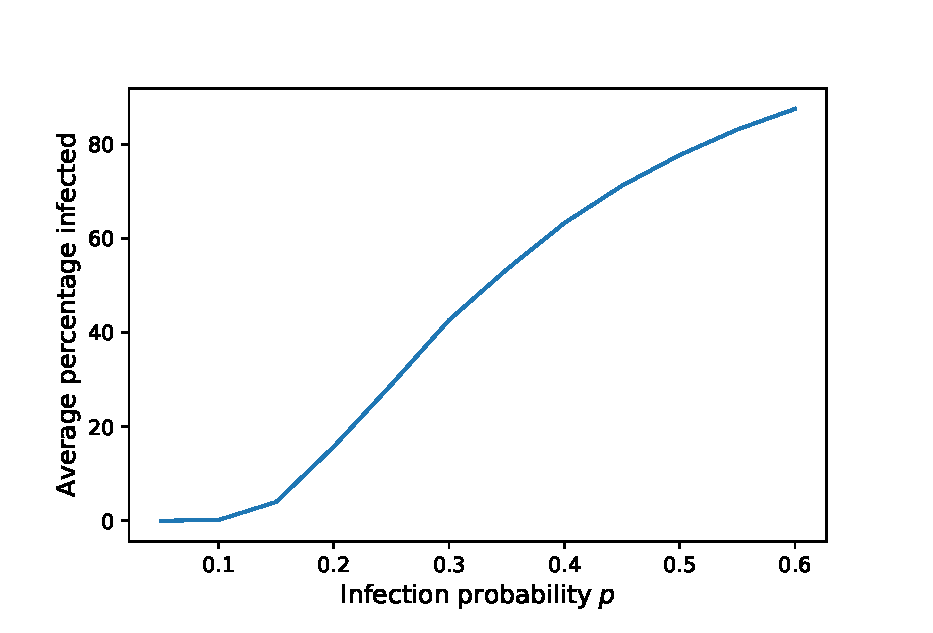
\includegraphics[scale = 0.55]{Figuresnew/PA_attackrates.eps}
    \caption{Preferential: p vs avg. percent infected.)}
    \label{fig:PA_ar}
\end{figure}

\begin{figure}[!h]
    \centering
    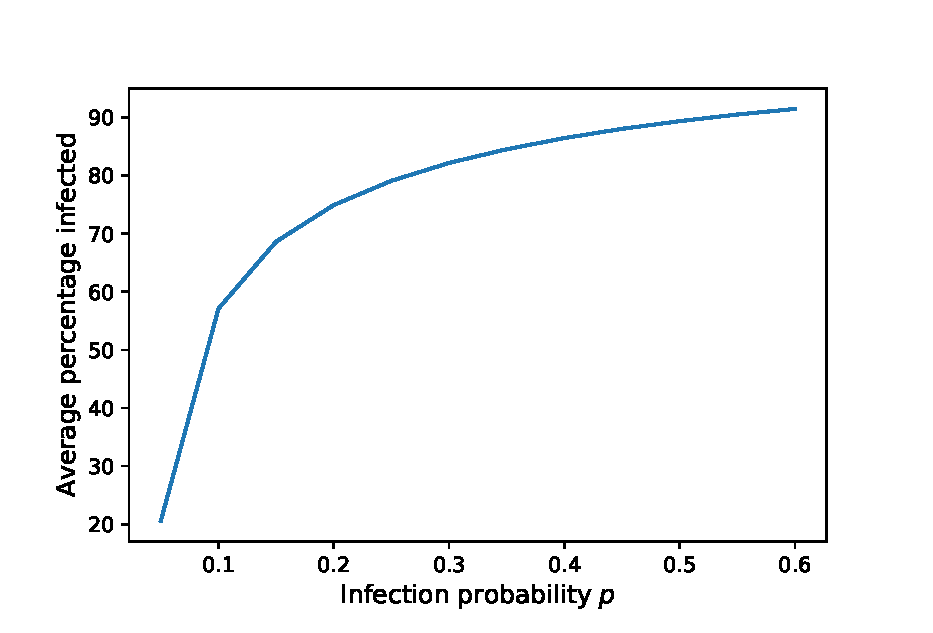
\includegraphics[scale = 0.55]{Figuresnew/montgo_attackrates.eps}
    \caption{Montgomery: p vs avg. percent infected.}
    \label{fig:montgo_ar}
\end{figure}



\begin{figure}[!h]
    \centering
    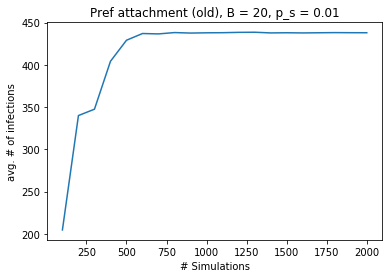
\includegraphics[scale = 0.6]{Figuresnew/simulations.png}
    \caption{Simulation vs average infected (Preferential Attachment)}
    \label{fig:pa_simvsavg}
\end{figure}
 
\begin{figure}[!h]
    \centering
    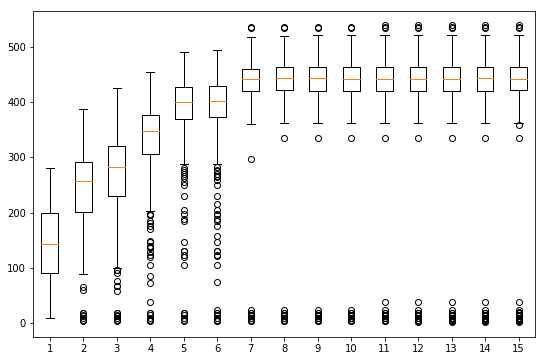
\includegraphics[scale = 0.4]{Figuresnew/boxplotpa.png}
    \caption{Box-plot: Simulation vs average infected (Preferential Attachment). X-axis: number of simulations (in 100s). Y-axis the number of infected.}
    \label{fig:pa_boxplot}
\end{figure}
\subsection{Performance Guarantees}
Will have plots for the larger datasets for both comparison with baselines and approximation guarantees.
\subsection{Pruning}
\begin{figure}[!h]
    \centering
    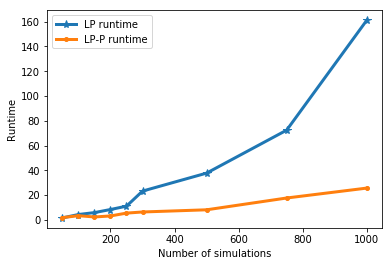
\includegraphics[scale = 0.55]{Figuresnew/pa1_runtime.png}
    \caption{Preferential1: Comparison of runtimes of Linear Programs with (LP-P) and without pruning (LP). }
    \label{fig:pa1pruningtime}
\end{figure}

\begin{figure}[!h]
    \centering
    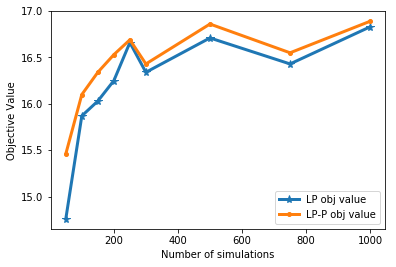
\includegraphics[scale = 0.55]{Figuresnew/pa1_objpruning.png}
    \caption{Preferential1: Comparison of of objective values of Linear Programs with (LP-P) and without pruning (LP). }
    \label{fig:pa1pruningobj}
\end{figure}


\subsubsection{Comparison to baselines}
\subsubsection{Approx Ratio}
\begin{figure}[!h]
    \centering
    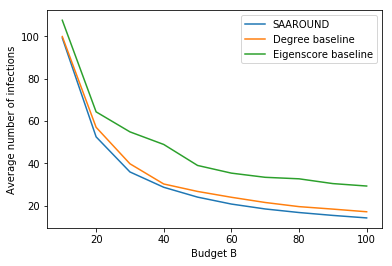
\includegraphics[scale = 0.55]{Figuresnew/pa1_obj.png}
    \caption{Preferential1: Comparison of \algo{} with the degree and eigenscore based baselines.}
    \label{fig:pa1approx}
\end{figure}

\begin{figure}[!h]
    \centering
    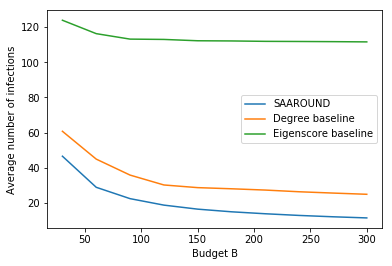
\includegraphics[scale = 0.55]{Figuresnew/pa2_obj.png}
    \caption{Preferential2: Comparison of \algo{} with the degree and eigenscore based baselines.}
    \label{fig:pa1approx}
\end{figure}

\begin{figure}[!h]
    \centering
    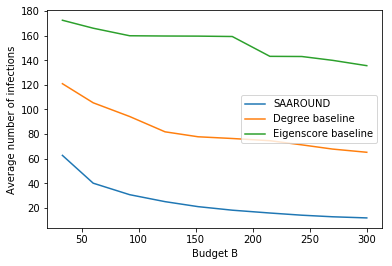
\includegraphics[scale = 0.55]{Figuresnew/mont_obj.png}
    \caption{Montgomery: Comparison of \algo{} with the degree and eigenscore based baselines.}
    \label{fig:pa1approx}
\end{figure}
\subsection{Two stage intervention and Structure of solution}
We study the two stage version of \prob{}. Here no information about the outbreak is available, and so, clearly, earlier is better, i.e., if the entire budget is available at time $0$, it is better to use it right away. In Figure \ref{fig:temporal}, we examine how the objective value $\expinf{}$ increases with $T$ in a two stage intervention, where $T$ is the time of the second stage. We observe that $\expinf{}$ increases very rapidly with $T$.

Next, we examine the structure of the sets picked in each stage. Figure \ref{fig:montagedeg} shows a scatter plot of the node degree and age of the solution to a two stage version with $T=4$. We observe that there are slight differences between the sets $X_0$ and $X_4$: $X_0$ has slightly higher degree nodes, whereas $X_4$ has slightly lower age nodes. But more importantly, \emph{it is not the case that all high degree nodes are used in $X_0$}.
\begin{figure}[!h]
    \centering
    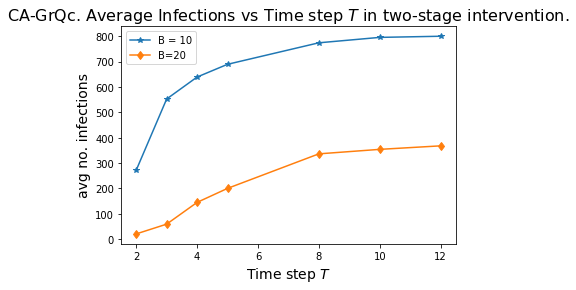
\includegraphics[scale = 0.45]{figures/twostage.png}
    \caption{CA-GrQc. Impact of varying $T$ in Two-stage Intervention. The X-axis corresponds to time step $T$ at which 2nd intervention is performed (1st intervention is at T =0). The Y-axis corresponds to the average number of infections over the simulations.}
    \label{fig:temporal}
\end{figure}

\begin{figure}[!h]
    \centering
    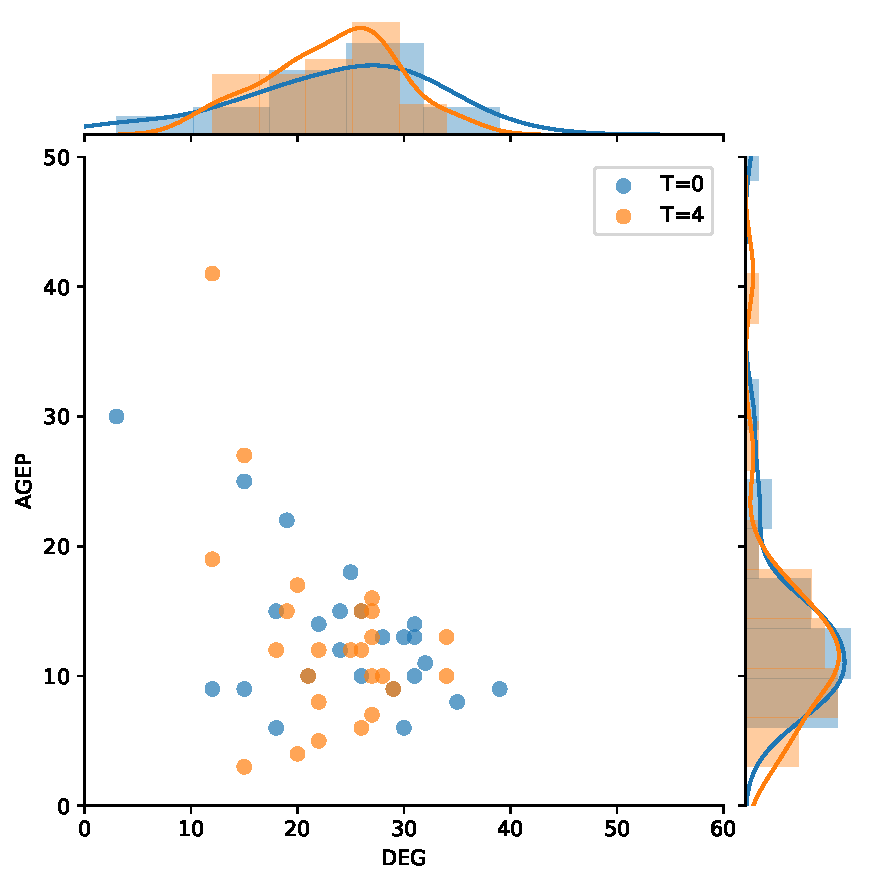
\includegraphics[scale = 0.45]{figures/t0_t4_compare_age_deg.pdf}
    \caption{Montgomery Graph: scatter plot of age and degree of nodes of the sets $X_0$ and $X_4$ in a solution to the 2-stage \prob{} with budgets $B_1 = B_4 = 25$.}
    \label{fig:montagedeg}
\end{figure}

\
%\subsection{Approximation Guarantees}


%\subsection{Characterizing Structure of Solution}

